% GNUPLOT: LaTeX picture with Postscript
\begingroup
  % Encoding inside the plot.  In the header of your document, this encoding
  % should to defined, e.g., by using
  % \usepackage[latin1,<other encodings>]{inputenc}
  \inputencoding{latin1}%
  \makeatletter
  \providecommand\color[2][]{%
    \GenericError{(gnuplot) \space\space\space\@spaces}{%
      Package color not loaded in conjunction with
      terminal option `colourtext'%
    }{See the gnuplot documentation for explanation.%
    }{Either use 'blacktext' in gnuplot or load the package
      color.sty in LaTeX.}%
    \renewcommand\color[2][]{}%
  }%
  \providecommand\includegraphics[2][]{%
    \GenericError{(gnuplot) \space\space\space\@spaces}{%
      Package graphicx or graphics not loaded%
    }{See the gnuplot documentation for explanation.%
    }{The gnuplot epslatex terminal needs graphicx.sty or graphics.sty.}%
    \renewcommand\includegraphics[2][]{}%
  }%
  \providecommand\rotatebox[2]{#2}%
  \@ifundefined{ifGPcolor}{%
    \newif\ifGPcolor
    \GPcolortrue
  }{}%
  \@ifundefined{ifGPblacktext}{%
    \newif\ifGPblacktext
    \GPblacktexttrue
  }{}%
  % define a \g@addto@macro without @ in the name:
  \let\gplgaddtomacro\g@addto@macro
  % define empty templates for all commands taking text:
  \gdef\gplbacktext{}%
  \gdef\gplfronttext{}%
  \makeatother
  \ifGPblacktext
    % no textcolor at all
    \def\colorrgb#1{}%
    \def\colorgray#1{}%
  \else
    % gray or color?
    \ifGPcolor
      \def\colorrgb#1{\color[rgb]{#1}}%
      \def\colorgray#1{\color[gray]{#1}}%
      \expandafter\def\csname LTw\endcsname{\color{white}}%
      \expandafter\def\csname LTb\endcsname{\color{black}}%
      \expandafter\def\csname LTa\endcsname{\color{black}}%
      \expandafter\def\csname LT0\endcsname{\color[rgb]{1,0,0}}%
      \expandafter\def\csname LT1\endcsname{\color[rgb]{0,1,0}}%
      \expandafter\def\csname LT2\endcsname{\color[rgb]{0,0,1}}%
      \expandafter\def\csname LT3\endcsname{\color[rgb]{1,0,1}}%
      \expandafter\def\csname LT4\endcsname{\color[rgb]{0,1,1}}%
      \expandafter\def\csname LT5\endcsname{\color[rgb]{1,1,0}}%
      \expandafter\def\csname LT6\endcsname{\color[rgb]{0,0,0}}%
      \expandafter\def\csname LT7\endcsname{\color[rgb]{1,0.3,0}}%
      \expandafter\def\csname LT8\endcsname{\color[rgb]{0.5,0.5,0.5}}%
    \else
      % gray
      \def\colorrgb#1{\color{black}}%
      \def\colorgray#1{\color[gray]{#1}}%
      \expandafter\def\csname LTw\endcsname{\color{white}}%
      \expandafter\def\csname LTb\endcsname{\color{black}}%
      \expandafter\def\csname LTa\endcsname{\color{black}}%
      \expandafter\def\csname LT0\endcsname{\color{black}}%
      \expandafter\def\csname LT1\endcsname{\color{black}}%
      \expandafter\def\csname LT2\endcsname{\color{black}}%
      \expandafter\def\csname LT3\endcsname{\color{black}}%
      \expandafter\def\csname LT4\endcsname{\color{black}}%
      \expandafter\def\csname LT5\endcsname{\color{black}}%
      \expandafter\def\csname LT6\endcsname{\color{black}}%
      \expandafter\def\csname LT7\endcsname{\color{black}}%
      \expandafter\def\csname LT8\endcsname{\color{black}}%
    \fi
  \fi
    \setlength{\unitlength}{0.0500bp}%
    \ifx\gptboxheight\undefined%
      \newlength{\gptboxheight}%
      \newlength{\gptboxwidth}%
      \newsavebox{\gptboxtext}%
    \fi%
    \setlength{\fboxrule}{0.5pt}%
    \setlength{\fboxsep}{1pt}%
\begin{picture}(8208.00,4464.00)%
    \gplgaddtomacro\gplbacktext{%
      \csname LTb\endcsname%%
      \put(377,594){\makebox(0,0){\fontsize{9}{9}\selectfont{4}}}%
      \put(377,960){\makebox(0,0){\fontsize{9}{9}\selectfont{6}}}%
      \put(377,1325){\makebox(0,0){\fontsize{9}{9}\selectfont{8}}}%
      \put(377,1691){\makebox(0,0){\fontsize{9}{9}\selectfont{10}}}%
      \put(377,2056){\makebox(0,0){\fontsize{9}{9}\selectfont{12}}}%
      \put(377,2422){\makebox(0,0){\fontsize{9}{9}\selectfont{14}}}%
      \put(377,2787){\makebox(0,0){\fontsize{9}{9}\selectfont{16}}}%
      \put(377,3153){\makebox(0,0){\fontsize{9}{9}\selectfont{18}}}%
      \put(377,3519){\makebox(0,0){\fontsize{9}{9}\selectfont{20}}}%
      \put(377,3884){\makebox(0,0){\fontsize{9}{9}\selectfont{22}}}%
      \put(694,396){\rotatebox{45}{\makebox(0,0)[l]{\strut{}\fontsize{7}{7}\selectfont{8,1}}}}%
      \put(927,396){\rotatebox{45}{\makebox(0,0)[l]{\strut{}\fontsize{7}{7}\selectfont{7,2}}}}%
      \put(1159,396){\rotatebox{45}{\makebox(0,0)[l]{\strut{}\fontsize{7}{7}\selectfont{6,3}}}}%
      \put(1391,396){\rotatebox{45}{\makebox(0,0)[l]{\strut{}\fontsize{7}{7}\selectfont{5,4}}}}%
      \put(1623,396){\rotatebox{45}{\makebox(0,0)[l]{\strut{}\fontsize{7}{7}\selectfont{4,5}}}}%
      \put(1856,396){\rotatebox{45}{\makebox(0,0)[l]{\strut{}\fontsize{7}{7}\selectfont{3,6}}}}%
      \put(2088,396){\rotatebox{45}{\makebox(0,0)[l]{\strut{}\fontsize{7}{7}\selectfont{2,7}}}}%
      \put(2320,396){\rotatebox{45}{\makebox(0,0)[l]{\strut{}\fontsize{7}{7}\selectfont{1,8}}}}%
      \put(2552,396){\rotatebox{45}{\makebox(0,0)[l]{\strut{}\fontsize{7}{7}\selectfont{8,0}}}}%
      \put(2785,396){\rotatebox{45}{\makebox(0,0)[l]{\strut{}\fontsize{7}{7}\selectfont{7,1}}}}%
      \put(3017,396){\rotatebox{45}{\makebox(0,0)[l]{\strut{}\fontsize{7}{7}\selectfont{6,2}}}}%
      \put(3249,396){\rotatebox{45}{\makebox(0,0)[l]{\strut{}\fontsize{7}{7}\selectfont{5,3}}}}%
      \put(3482,396){\rotatebox{45}{\makebox(0,0)[l]{\strut{}\fontsize{7}{7}\selectfont{4,4}}}}%
      \put(3714,396){\rotatebox{45}{\makebox(0,0)[l]{\strut{}\fontsize{7}{7}\selectfont{3,5}}}}%
      \put(3946,396){\rotatebox{45}{\makebox(0,0)[l]{\strut{}\fontsize{7}{7}\selectfont{2,6}}}}%
      \put(4178,396){\rotatebox{45}{\makebox(0,0)[l]{\strut{}\fontsize{7}{7}\selectfont{1,7}}}}%
      \put(4411,396){\rotatebox{45}{\makebox(0,0)[l]{\strut{}\fontsize{7}{7}\selectfont{0,8}}}}%
      \put(4643,396){\rotatebox{45}{\makebox(0,0)[l]{\strut{}\fontsize{7}{7}\selectfont{7,0}}}}%
      \put(4875,396){\rotatebox{45}{\makebox(0,0)[l]{\strut{}\fontsize{7}{7}\selectfont{6,1}}}}%
      \put(5107,396){\rotatebox{45}{\makebox(0,0)[l]{\strut{}\fontsize{7}{7}\selectfont{5,2}}}}%
      \put(5340,396){\rotatebox{45}{\makebox(0,0)[l]{\strut{}\fontsize{7}{7}\selectfont{4,3}}}}%
      \put(5572,396){\rotatebox{45}{\makebox(0,0)[l]{\strut{}\fontsize{7}{7}\selectfont{3,4}}}}%
      \put(5804,396){\rotatebox{45}{\makebox(0,0)[l]{\strut{}\fontsize{7}{7}\selectfont{2,5}}}}%
      \put(6037,396){\rotatebox{45}{\makebox(0,0)[l]{\strut{}\fontsize{7}{7}\selectfont{1,6}}}}%
      \put(6269,396){\rotatebox{45}{\makebox(0,0)[l]{\strut{}\fontsize{7}{7}\selectfont{0,7}}}}%
      \put(6501,396){\rotatebox{45}{\makebox(0,0)[l]{\strut{}\fontsize{7}{7}\selectfont{6,0}}}}%
      \put(6733,396){\rotatebox{45}{\makebox(0,0)[l]{\strut{}\fontsize{7}{7}\selectfont{5,1}}}}%
      \put(6966,396){\rotatebox{45}{\makebox(0,0)[l]{\strut{}\fontsize{7}{7}\selectfont{4,2}}}}%
      \put(7198,396){\rotatebox{45}{\makebox(0,0)[l]{\strut{}\fontsize{7}{7}\selectfont{3,3}}}}%
      \put(7430,396){\rotatebox{45}{\makebox(0,0)[l]{\strut{}\fontsize{7}{7}\selectfont{2,4}}}}%
      \put(7662,396){\rotatebox{45}{\makebox(0,0)[l]{\strut{}\fontsize{7}{7}\selectfont{1,5}}}}%
      \put(7895,396){\rotatebox{45}{\makebox(0,0)[l]{\strut{}\fontsize{7}{7}\selectfont{0,6}}}}%
      \put(4361,4298){\makebox(0,0){\strut{}\fontsize{13}{13}\selectfont{Resultados en mallas de 3 $\times$ 3}}}%
      \put(4361,110){\makebox(0,0){\strut{}\fontsize{12}{12}\selectfont{Objetos en malla (cubos, prismas)}}}%
      \put(66,2331){\rotatebox{90}{\makebox(0,0){\strut{}\fontsize{12}{12}\selectfont{Costo global $T$}}}}%
      \put(7810,3424){\makebox(0,0)[l]{\strut{}}}%
      \csname LTb\endcsname%%
      \put(7963,3424){\makebox(0,0)[l]{\strut{}}}%
      \csname LTb\endcsname%%
      \put(7833,3411){\makebox(0,0)[l]{\strut{}\fontsize{8}{8}\selectfont{,}}}%
    }%
    \gplgaddtomacro\gplfronttext{%
      \csname LTb\endcsname%%
      \put(7598,3853){\makebox(0,0)[r]{\strut{}\fontsize{8}{8}\selectfont{B\'usqueda exhaustiva}}}%
      \csname LTb\endcsname%%
      \put(7598,3633){\makebox(0,0)[r]{\strut{}\fontsize{8}{8}\selectfont{B\'usqueda por RS}}}%
      \csname LTb\endcsname%%
      \put(7598,3413){\makebox(0,0)[r]{\strut{}\fontsize{8}{8}\selectfont{Costo global \'optimo}}}%
    }%
    \gplbacktext
    \put(0,0){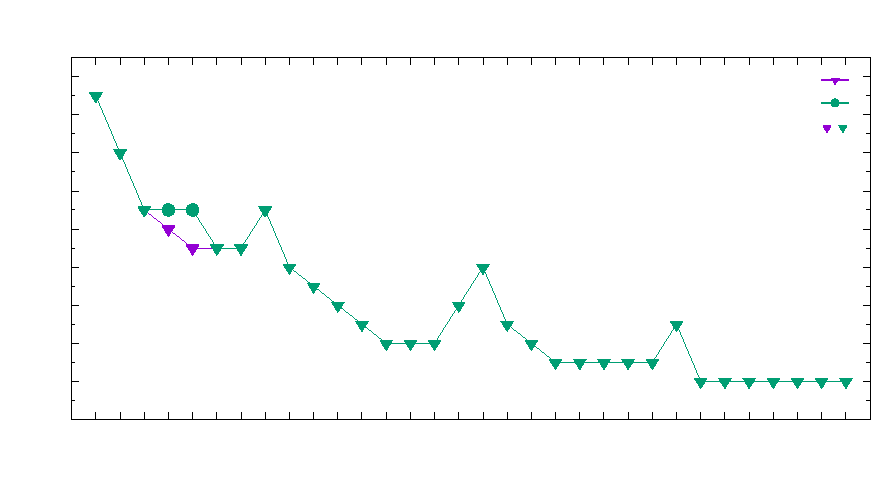
\includegraphics{resultados_3x3}}%
    \gplfronttext
  \end{picture}%
\endgroup
